% !TeX spellcheck = en_US
This little quick tour from here: \href{https://www.carbon111.com/xt_intro.html}{Carbon111}
\subsection{A Quick Tour of the MicrowaveII/XT}
If you need a quick introduction to the Microwave II/XT or just want to know what all the fuss is about, here you go.
Welcome to my quick tour of the Microwave II/XT/XTk (for simplicity's sake hereafter refered to as the XT). If you are familiar with Subtractive Analog synthesis then you will readily understand the XT. First, lets look at a block diagram of how the WaveXT is laid out - this will be our "roadmap":
A complete answer for just reference.
\bigskip % Add an empty line
%These are optional parameters to finetune the placement of tables and figures, with the following meaning:
%
%h, here
%t, top
%b, bottom
%p, page of float
%e.g. \begin{figure}[!htb]
\begin{figure}[ht!]
	\centering
	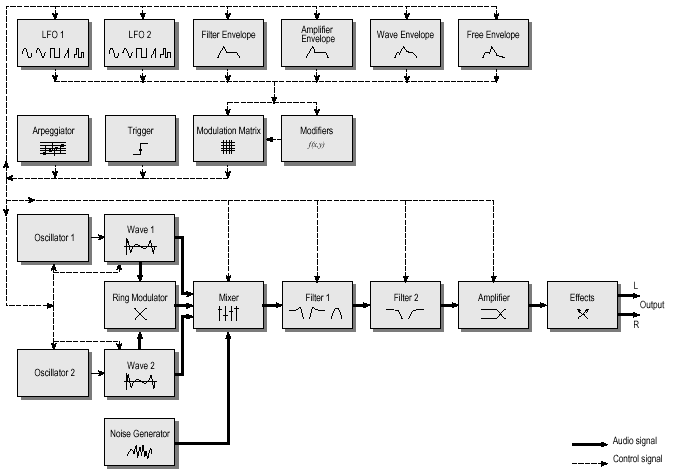
\includegraphics[width=90mm]{pics/mwxt_block.png}
	\caption{Microwave II block diagram}
	\label{blockdiagrammwxt}
\end{figure}
\paragraph{Oscillators and Wavetables}
Our First stop is the Oscillators. The XT has two of these. Unlike a standard analog synthesizer, the oscillators aren't heard directly - they merely drive the frequency of the waveform generators for the currently chosen wavetable. If this doesn't make sense immediately, don't worry about it, just remember that the oscillators drive the pitch of the currently chosen wavetable wave. The oscillators and wavetabes (and, for that matter, even the filters) of this synth make no apologies about being unabashedly digital.\\
Wavetable synthesis is characterized by the ability to sequence through a table of different waveforms during the duration of a single note. The XT has 65 preset wavetables and 32 user-programmable wavetables. A wavetable can be pictured as a row of 64 pointers to any of the 300 waveforms stored in the XT's ROM memory or any waveforms available in the user memory. Lets look at wavetable 016 "Square Saw" as an example:
\begin{figure}[ht!]
	\centering
	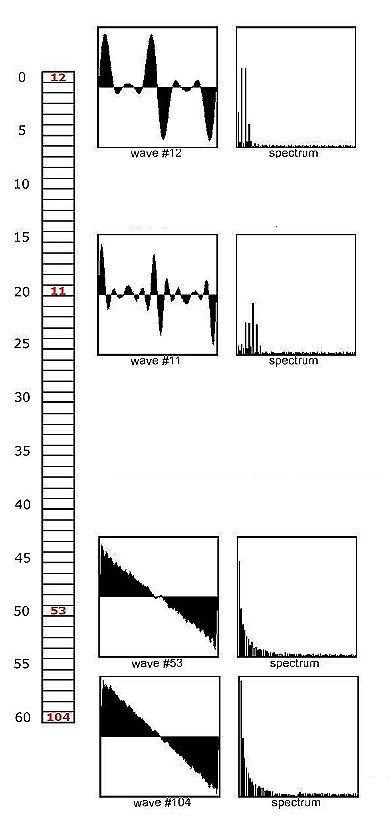
\includegraphics[width=90mm]{pics/osc_wt.jpg}
	\caption{pointers and wavetable with spectrum}
	\label{osc_wt}
\end{figure}
At position 0 is a pointer to ROM waveform \#12, a waveform with strong 2nd and 3rd harmonics, vaguely reminiscent of a square wave. The next pointer is at position 20 for ROM wave \#11, similar to \#12 but with higher harmonics. Next at position 50 is ROM wave \#53, very close to a sawtooth wave. Finally at position 60 is ROM wave \#104, a familiar classic ``buzzy'' sawtooth. The table positions from 1 - 19, 21 - 49 and 51 - 59 are interpolated by the XT automatically. If you move the start wave up or down the wavetable with an envelope, LFO or even the modwheel, you get a smooth transition between each of the four ``real'' waveforms because of the crossfading or "morphing" caused by the XT's interpolation to fill in the gaps.\\
So, if you were to set up a simple sound with just one oscillator with an initial start wave setting of 0 and a basic ramp envelope controlling wavetable position, when you struck a key, you would get a smooth sweep from a ``squarish-sounding'' wave \#12 all the way to a bright "buzzy" sawtooth wave \#103 without any gaps or glitches in between. Of course we are not limited to gentle sweeps with simple ramp EGs - we can use the powerful 8-time 8-level wave envelope generator with its sustain and release loops to create unique and complex timbral morphs if we want - and we do want!\\
The last three positions in each wavetable (61, 62 \& 63) are always reserved for the classic analog subtractive synth waveforms: saw, square and triangle so they are always available if needed. We can turn on a ``limit'' function for the oscillators so we don't unintentionally stray onto the analog waves when scanning the wavetable - a handy feature to avoid timbral glitches. Some of the wavetables in the XT emulate different types of filter sweeps, others offer simulated pulse width modulation, formant sweeps and other timbral morphs. These are designed to be swept with an envelope, LFO or smooth modulator of your choice. Other wavetables like 064 ``Chorus2'' are designed instead to make use of the keytrack parameter to keep a homophonic timbre across a number of octaves - changing the waveform depending on the key played. Still, other wavetables, like the four ``Wavetrip'' tables, are diverse collections of disparate waves well suited to creative cacophony and euphony of all kinds.\\
Hardwired to the wave position parameter of waveform generators 1 and 2 is the so-called wave envelope which is a very powerful 8-time 8-level complex envelope with user-adjustable looping points in the sustain and release segments. This envelope can be used to modulate other elements in the XT too through the modmatrix - more on that later.\\
Ring modulation, hard sync and glide are available for even more oscillator mayhem but lest we dwell too long at the start of our trip we forge on...
\paragraph{Filters}
Next on our journey are the filters. The XT is outfitted with two filters set up in series. The second filter is a basic 6dB filter switchable between lowpass or highpass - mainly used to ``tidy up'' the output of the first filter. The main filter on the XT is an amazing multimode beast with 10 different filter types - lets look at some of the more interesting possibilities:
\begin{itemize}
	\item 24dB and 12dB Lowpass: These are the ``classic'' analog-style filters used for most subtractive synthesis. The 24dB gives an ``aggressive'' filtered sound reminiscent of a Moog ``ladder'' while the 12dB offers a much softer slope much like the old Oberheim synths. Even though the XT is no ``virtual analog'', the filters can be very convincing depending on the application. 
	\item Sine Waveshaper and 12dB Lowpass: This filter packs a real punch with a tight compression sound provided by the sine waveshaper. Excellent on bass sounds.
	\item Waveshaper: This filter has some real suprises, similar to the Sine Waveshaper but with the ability to use any wave in the current wavetable as the shaper wave! Used with a square wave, this filter will rip your face off.
	\item Dual Lowpass/Bandpass: This is a dual filter combining a 12dB lowpass with a 12dB bandpass in series. Sweep different cutoff settings for each filter from different modulators to get amazing shimmering, ``swirling-in-front-of-your-face'' type sounds.
	\item S/H (Sample \& Hold) into 12dB Lowpass: This filter is a brutal sample-rate reduction processor combined with a standard 12dB lowpass. Make the XT sound like a really crappy, cheap low-res sampler! This is a good thing!
	\item There are six other filters as well but I will let you discover those for yourself.
\end{itemize}
Hardwired to the Filter is a basic ADSR envelope that can be used with or overridden by any modulation you choose. Modulating decay time with key velocity is a nice touch for instance.
\paragraph{Amplifier \& Pan}
Pretty basic but you gotta have it. An amp with its own hardwired ADSR feeds directly into a panning circuit. You can modulate pan position with a modulator of your choosing - a random S/H waveform is one of my favorites. Next...
\paragraph{Modulation Matrix}
Here lies the element that pulls all this power into a cohesive force! The modulation matrix allows you to route any of 32 modulation sources to any of 43 destinations! Sources include any of the XT's four envelopes, two LFOs, wheels, pressure, keytrack, etc. Destinations include wave position, pitch, amp levels, LFO rate, volume, panning, cutoff, resonance, you-name-it! You can also do an end-run around any of the XT's hardwiring and, for example, use the wave envelope to control the filter cutoff and the filter envelope to control pan position.
\paragraph{Other}
Yes, I know there's much more - but this was a quick tour, remember. If you still want to know more about the XT, download the User Manual or check out Waldorf's "Additional Information" page. Better yet, try one out! \todo{Add literature references}